 
\documentclass[12pt, a4paper]{article}
\usepackage{graphicx}
\usepackage{mathtools}
\usepackage{xcolor}
\usepackage{amsmath}
\usepackage{caption}
\usepackage[italian]{babel}
\usepackage{eso-pic}
\usepackage{setspace}
\usepackage{multirow}
\usepackage{array}
\usepackage{geometry}
\usepackage{longtable}
\graphicspath{ {./immagini/} }
\linespread{1.1}
\geometry{
 total={170mm,257mm},
 left=20mm,
 top=15mm,
 bottom=28mm
 }
 
 \title{\textbf{\scalebox{1.3}{\text{Caduta libera}}}}
 \date{}

\begin{document}
\maketitle
\AddToShipoutPictureBG*{%
  \AtPageUpperLeft{%
    \hspace{\paperwidth}%
    \raisebox{-\baselineskip}{%
      \makebox[0pt][r]{\textbf{Gruppo 10}: Mussini Simone, Musi Francesco, Ruscillo Fabio        }
}}}%

\section{Fenomeno fisico}
Il fenomeno della caduta libera è dovuto alla forza di attrazione gravitazionale, descritta dalla legge seguente, valida per qualsiasi coppia di enti dotati di massa: 


\begin{equation*}
    \Vec{F_g} = -G\frac{M m}{r^2}\ \hat{r}
\end{equation*}
Con G costante di gravitazione universale, $M$ e $m$ le masse dei due corpi ed $r$ la distanza tra essi.

Per questa forza è possibile definire un campo, detto campo gravitazionale, indicato con la lettera $\Vec{g}$. 
Il concetto di campo rappresenta come varia la forza generata da un corpo in funzione della distanza, e si presenta come: 

\begin{equation*}
    \Vec{g}(r) = -G\frac{M}{r^2}\  \hat{r}
\end{equation*}

Data questa definizione, l'espressione della forza diventa $\Vec{F_g} = \Vec{g}(r)m$. 
Ricordando la seconda legge della dinamica, notiamo subito che \textit{il campo $\Vec{g}(r)$ rappresenta l'accelerazione con cui un corpo di massa $m$ viene attratto verso un altro corpo di massa $M$.} 
Il termine "accelerazione di gravità" deriva proprio da ciò.

Il suo valore, adottato sulla Terra, è quello che si ottiene dall'espressione $\displaystyle {g(R_t) = G\frac{M_t}{R_t^2}}$, usando la massa terrestre $M_t$ ed il valore medio del raggio terrestre $R_t$ poichè la Terra non è perfettamente sferica, ed è pari a $g_{tab}=(9.80665\pm 0.00001)\ m/s^2$.

Se la distanza del corpo rispetto alla superficie terrestre è molto minore di $R_t$, basta moltiplicare la massa $m$ dell'oggetto e il valore $g_{tab}$, per ottenere la forza con cui la Terra e il corpo si attraggono a vicenda.

Si possono considerare trascurabili le forze di attrazione con oggetti minori, come ad esempio il tavolo su cui si svolge l'esperimento, perchè essi generano forze assolutamente irrilevanti rispetto a quella di attrazione terrestre.

\section{Obbiettivo}
\label{sezione obbiettivi}
Lo scopo di questo esperimento è di riuscire ad ottenere la misura dell'accelerazione di gravità, analizzando un filmato che ritrae una sferetta in caduta libera. 
Ciò è stato fatto prendendo varie misure della posizione del corpo tramite fotoregistrazioni ad alta velocità. 

La formula da usare, che mette in relazione $g$ e la posizione del corpo, è:
\begin{equation*}
    y(t) = \frac{1}{2}gt^2+ v(0)t+y(0)
\end{equation*}


\section{Strumenti}
\begin{itemize}
\setlength\itemsep{0mm}
    \item Programma di analisi "\textit{Tracker}"
    \item Video con 1000 fotogrammi al secondo
\end{itemize}

\section{Procedimento di misura}
Il setup dell'esperimento, osservabile nel video, comprende un asta, alla sommità della quale è posizionata una sferetta metallica ferma. L'asta presenta dei segni distanziati gli uni dagli altri di 10cm. 
Ad un certo punto la sferetta viene rilasciata e cade muovendosi di moto uniformemente accelerato, soggetta alla sola forza peso. Affianco all'asta è presente un cronometro con sensibilità al millesimo di secondo. 
Essendo il tutto filmato da una fotocamera (\textit{Sony DSC-RX100M4}) che registra a 1000\textit{fps}, ad ogni frame il cronometro avanza di un millesimo di secondo.

  
\subsection{Setting del programma di tracciamento}
Per iniziare, mediante la funzione "\textit{asta di calibrazione}", si è posto uguale a 10cm la distanza tra 2 segni sull'asta, in modo che il programma potesse generare un metro calibrato con cui misurare la posizione del target. Il metro calibrato, è poi stato posto in modo che l'origine coincidesse con la posizione del primo punto di massa, posizionato alla base della sferetta a riposo. Poi si è stabilito il frame di inizio del moto della sferetta, che è risultato essere il 49esimo. 

La posizione è stata segnata ogni 10 frame, ponendo, ad ogni misura, i punti di massa nella parte inferiore della sferetta. 

In totale sono state prese 42 misure.


\subsection{Gestione degli errori sulle misure}
L'alta velocità di acquisizione della fotocamera è a scapito della quantità di luce catturata, quindi anche della nitidezza dell'immagine.
Gli errori sono stati scelti in base al numero di pixel di transizione tra il colore del target e dello sfondo, e sono stati stimati misura per misura, visto che la nitidezza di ogni frame era variabile. Tramite il metro di calibrazione è stato posto: 1$px$ = $(0.0005\pm 0.0001)$ $m$, pertanto:
\begin{equation*}
    \Delta y_{mis}= (n^o pixel \cdot 0.0005)m
\end{equation*}
Di seguito è riportata la tabella dei dati misurati per via diretta e indiretta.
\newpage

\section{Tabella dei dati misurati}
\begin{table}[!h]
    \centering
\centerline{\begin{tabular}{|c|c|c|c|}
    \hline
    \multirow{2}{*}{\small Misura} &
    \multirow{2}{*}{ \small$y_{mis}\pm \Delta y_{mis}$\ $(m)$}&
    \multirow{2}{*}{\small $n^o pixel$}&
    \multirow{2}{*}{\small $t\pm \Delta t\ (s)$}\\
    &&&\\ 
\hline
\hline
\footnotesize$1$  & \footnotesize$0.0001 \pm 0.0010$ & \footnotesize$2$ & \footnotesize$0.012\pm 0.001$\\ 
\footnotesize$2$  & \footnotesize$0.0020 \pm 0.0010$ & \footnotesize$2$ & \footnotesize$0.022\pm 0.001$\\
\footnotesize$3$  & \footnotesize$0.0045 \pm 0.0015$ & \footnotesize$3$ & \footnotesize$0.032\pm 0.001$\\
\footnotesize$4$  & \footnotesize$0.0090 \pm 0.0015$ & \footnotesize$3$ & \footnotesize$0.042\pm 0.001$\\
\footnotesize$5$  & \footnotesize$0.0130 \pm 0.0015$ & \footnotesize$3$ & \footnotesize$0.052\pm 0.001$\\
\footnotesize$6$  & \footnotesize$0.0195 \pm 0.0015$ & \footnotesize$3$ & \footnotesize$0.062\pm 0.001$\\
\footnotesize$7$  & \footnotesize$0.0250 \pm 0.0020$ & \footnotesize$4$ & \footnotesize$0.072\pm 0.001$\\
\footnotesize$8$  & \footnotesize$0.0325 \pm 0.0020$ & \footnotesize$4$ & \footnotesize$0.082\pm 0.001$\\
\footnotesize$9$  & \footnotesize$0.0420 \pm 0.0015$ & \footnotesize$3$ & \footnotesize$0.092\pm 0.001$\\
\footnotesize$10$ & \footnotesize$0.0515 \pm 0.0015$ & \footnotesize$3$ & \footnotesize$0.102\pm 0.001$\\
\footnotesize$11$ & \footnotesize$0.0620 \pm 0.0010$ & \footnotesize$2$ & \footnotesize$0.112\pm 0.001$\\
\footnotesize$12$ & \footnotesize$0.0730 \pm 0.0020$ & \footnotesize$4$ & \footnotesize$0.122\pm 0.001$\\   
\footnotesize$13$ & \footnotesize$0.0865 \pm 0.0020$ & \footnotesize$4$ & \footnotesize$0.132\pm 0.001$\\
\footnotesize$14$ & \footnotesize$0.1005 \pm 0.0015$ & \footnotesize$3$ & \footnotesize$0.142\pm 0.001$\\
\footnotesize$15$ & \footnotesize$0.1160 \pm 0.0010$ & \footnotesize$2$ & \footnotesize$0.152\pm 0.001$\\
\footnotesize$16$ & \footnotesize$0.1315 \pm 0.0020$ & \footnotesize$4$ & \footnotesize$0.162\pm 0.001$\\
\footnotesize$17$ & \footnotesize$0.1475 \pm 0.0015$ & \footnotesize$3$ & \footnotesize$0.172\pm 0.001$\\
\footnotesize$18$ & \footnotesize$0.1660 \pm 0.0015$ & \footnotesize$3$ & \footnotesize$0.182\pm 0.001$\\
\footnotesize$19$ & \footnotesize$0.1850 \pm 0.0015$ & \footnotesize$3$ & \footnotesize$0.192\pm 0.001$\\
\footnotesize$20$ & \footnotesize$0.2045 \pm 0.0020$ & \footnotesize$4$ & \footnotesize$0.202\pm 0.001$\\ 
\footnotesize$21$ & \footnotesize$0.2250 \pm 0.0005$ & \footnotesize$1$ & \footnotesize$0.212\pm 0.001$\\
\footnotesize$22$ & \footnotesize$0.2465 \pm 0.0010$ & \footnotesize$2$ & \footnotesize$0.222\pm 0.001$\\
\footnotesize$23$ & \footnotesize$0.2700 \pm 0.0010$ & \footnotesize$2$ & \footnotesize$0.232\pm 0.001$\\
\footnotesize$24$ & \footnotesize$0.2935 \pm 0.0020$ & \footnotesize$4$ & \footnotesize$0.242\pm 0.001$\\
\footnotesize$25$ & \footnotesize$0.3180 \pm 0.0015$ & \footnotesize$3$ & \footnotesize$0.252\pm 0.001$\\ 
\footnotesize$26$ & \footnotesize$0.3435 \pm 0.0010$ & \footnotesize$2$ & \footnotesize$0.262\pm 0.001$\\
\footnotesize$27$ & \footnotesize$0.3700 \pm 0.0020$ & \footnotesize$4$ & \footnotesize$0.272\pm 0.001$\\
\footnotesize$28$ & \footnotesize$0.3975 \pm 0.0015$ & \footnotesize$3$ & \footnotesize$0.282\pm 0.001$\\
\footnotesize$29$ & \footnotesize$0.4260 \pm 0.0010$ & \footnotesize$2$ & \footnotesize$0.292\pm 0.001$\\
\footnotesize$30$ & \footnotesize$0.4550 \pm 0.0010$ & \footnotesize$2$ & \footnotesize$0.302\pm 0.001$\\
\footnotesize$31$ & \footnotesize$0.4865 \pm 0.0015$ & \footnotesize$3$ & \footnotesize$0.312\pm 0.001$\\
\footnotesize$32$ & \footnotesize$0.5180 \pm 0.0010$ & \footnotesize$2$ & \footnotesize$0.322\pm 0.001$\\
\footnotesize$33$ & \footnotesize$0.5500 \pm 0.0015$ & \footnotesize$3$ & \footnotesize$0.332\pm 0.001$\\
\footnotesize$34$ & \footnotesize$0.5835 \pm 0.0015$ & \footnotesize$3$ & \footnotesize$0.342\pm 0.001$\\
\footnotesize$35$ & \footnotesize$0.6175 \pm 0.0010$ & \footnotesize$2$ & \footnotesize$0.352\pm 0.001$\\
\footnotesize$36$ & \footnotesize$0.6520 \pm 0.0020$ & \footnotesize$4$ & \footnotesize$0.362\pm 0.001$\\
\footnotesize$37$ & \footnotesize$0.6875 \pm 0.0015$ & \footnotesize$3$ & \footnotesize$0.372\pm 0.001$\\
\footnotesize$38$ & \footnotesize$0.7245 \pm 0.0015$ & \footnotesize$3$ & \footnotesize$0.382\pm 0.001$\\
\footnotesize$39$ & \footnotesize$0.7625 \pm 0.0015$ & \footnotesize$3$ & \footnotesize$0.392\pm 0.001$\\ 
\footnotesize$40$ & \footnotesize$0.8020 \pm 0.0020$ & \footnotesize$4$ & \footnotesize$0.402\pm 0.001$\\
\footnotesize$41$ & \footnotesize$0.8420 \pm 0.0010$ & \footnotesize$2$ & \footnotesize$0.412\pm 0.001$\\ 
\footnotesize$42$ & \footnotesize$0.8835 \pm 0.0010$ & \footnotesize$2$ & \footnotesize$0.422\pm 0.001$\\ 
\hline
    \end{tabular}}
  \caption{\begin{footnotesize}Sono riportati in Tabella le posizioni misurate $y_{mis}$ col rispettivo errore $\Delta y_{mis}$ ottenuto a partire dal $n^o pixel$, ed il tempo corrispettivo di ogni posizione, avente come errore la sensibilità del cronometro.\end{footnotesize}}
  \label{Tabella Completa}
\end{table}
\newpage
\section{Considerazioni preliminari}

\subsection{Tempo di caduta}
Il frame di inizio della caduta è il 49\textit{esimo}, che corrisonde ad un tempo iniziale \textit{$t_i = (0.012\pm 0.001)\ s$}.
Abbiamo poi terminato lo studio del moto al 459esimo fotogramma, che corrisponde all'istante \textit{$t_f = (0.422\pm 0.001)\ s$}, per un tempo totale di caduta \textit{$(t_f-t_i) = (0.410\pm 0.002)\ s$}.
E' stato scelto come ultimo istante di caduta, quello che corrisponde all'ultima misura utile, appena precedente al rimbalzo della pallina sul banco di lavoro.\\
\subsection{Stima dell'ordine di grandezza di $g$}
Per avere una stima preliminare sull'ordine di grandezza dell'errore su $g$, sono stati calcolati gli errori relativi di una posizione e di un tempo centrali nelle misure. Siano $y_{mediano}=(0.2465\pm0.0010)$\ , e \ $t_{mediano}=(0.033\pm0.001)$ :
\begin{equation*}
    \frac{\Delta g}{g}=\frac{\Delta y_{mediano}}{y_{mediano}}+2\cdot \frac{\Delta t_{mediano}}{t_{mediano}}
\end{equation*}

Otteniamo che $\displaystyle\frac{\Delta g}{g}\approx 6\%$.\bigskip\\
\subsection{Correzione dell'errore sulla posizione}
Poichè la posizione dipende dal tempo, e l'ordine di grandezza degli errori relativi di
$\displaystyle{\frac{\Delta y_{mis}}{y_{mis}}}$ e $\displaystyle{\frac{\Delta t}{t}}$ è lo stesso per la maggior parte delle misure, si calcola un nuovo errore su $y_{mis}$ pari a 
\begin{equation*}
   \Delta y^{'} = \left(\frac{2\Delta t}{t}\right)\cdot y + \Delta y_{mis}
\end{equation*}

\begin{longtable}{|c|c|}
    \hline
    \multirow{2}{*}{\small Misura} &
    \multirow{2}{*}{ \small$\Delta y^{'}$\ $(m)$} 
    \\&\\
\hline
\hline
\footnotesize$1$  & \footnotesize$0.001 $ \\
\footnotesize$2$  & \footnotesize$0.001$ \\
\footnotesize$3$  & \footnotesize$0.002 $ \\
\footnotesize$4$  & \footnotesize$0.002 $ \\
\footnotesize$5$  & \footnotesize$0.002 $ \\
\footnotesize$6$  & \footnotesize$0.002 $ \\ 
\footnotesize$7$  & \footnotesize$0.003 $ \\
\footnotesize$8$  & \footnotesize$0.003 $ \\
\footnotesize$9$  & \footnotesize$0.002 $ \\
\footnotesize$10$ & \footnotesize$0.003 $ \\ 
\footnotesize$11$ & \footnotesize$0.002 $ \\
\hline
\footnotesize$12$ & \footnotesize$0.003 $ \\    
\footnotesize$13$ & \footnotesize$0.003 $ \\
\footnotesize$14$ & \footnotesize$0.003 $ \\
\footnotesize$15$ & \footnotesize$0.004 $ \\
\footnotesize$16$ & \footnotesize$0.004 $ \\
\footnotesize$17$ & \footnotesize$0.003 $ \\
\footnotesize$18$ & \footnotesize$0.003 $ \\
\footnotesize$19$ & \footnotesize$0.003 $ \\
\footnotesize$20$ & \footnotesize$0.004 $ \\ 
\footnotesize$21$ & \footnotesize$0.003 $ \\
\footnotesize$22$ & \footnotesize$0.003 $ \\
\footnotesize$23$ & \footnotesize$0.003 $ \\
\footnotesize$24$ & \footnotesize$0.004 $ \\
\footnotesize$25$ & \footnotesize$0.004 $ \\ 
\footnotesize$26$ & \footnotesize$0.004 $ \\
\footnotesize$27$ & \footnotesize$0.005 $ \\
\footnotesize$28$ & \footnotesize$0.004 $ \\
\footnotesize$29$ & \footnotesize$0.004 $ \\
\footnotesize$30$ & \footnotesize$0.004 $ \\
\footnotesize$31$ & \footnotesize$0.005 $ \\
\footnotesize$32$ & \footnotesize$0.004 $ \\
\footnotesize$33$ & \footnotesize$0.005 $ \\
\footnotesize$34$ & \footnotesize$0.005 $ \\
\footnotesize$35$ & \footnotesize$0.005 $ \\
\footnotesize$36$ & \footnotesize$0.006 $ \\
\footnotesize$37$ & \footnotesize$0.005 $ \\
\footnotesize$38$ & \footnotesize$0.005 $ \\
\footnotesize$39$ & \footnotesize$0.006 $ \\
\footnotesize$40$ & \footnotesize$0.005 $ \\
\footnotesize$41$ & \footnotesize$0.005 $ \\ 
\footnotesize$42$ & \footnotesize$0.005 $ \\ 
\hline
\caption{\begin{footnotesize}
            E' riportato in Tabella l'errore corretto sulla posizione $\Delta y^'$.
         \end{footnotesize}}
  
  \label{Tabella Completa}
\end{longtable}
\newpage

\section{Regressione di potenza} \label{Agg. misure xconcl}
Il primo grafico realizzato con il programma di analisi dati \textit{Igor Pro}, è stato il grafico spazio-tempo, che dovrebbe seguire la legge oraria del Paragrafo \ref{sezione obbiettivi}: \textit{Obbiettivi} (traiettoria parabolica con posizione $y(0)$ e velocità $v(0)$ iniziali nulle): 

    \begin{figure}[h!]
\centering
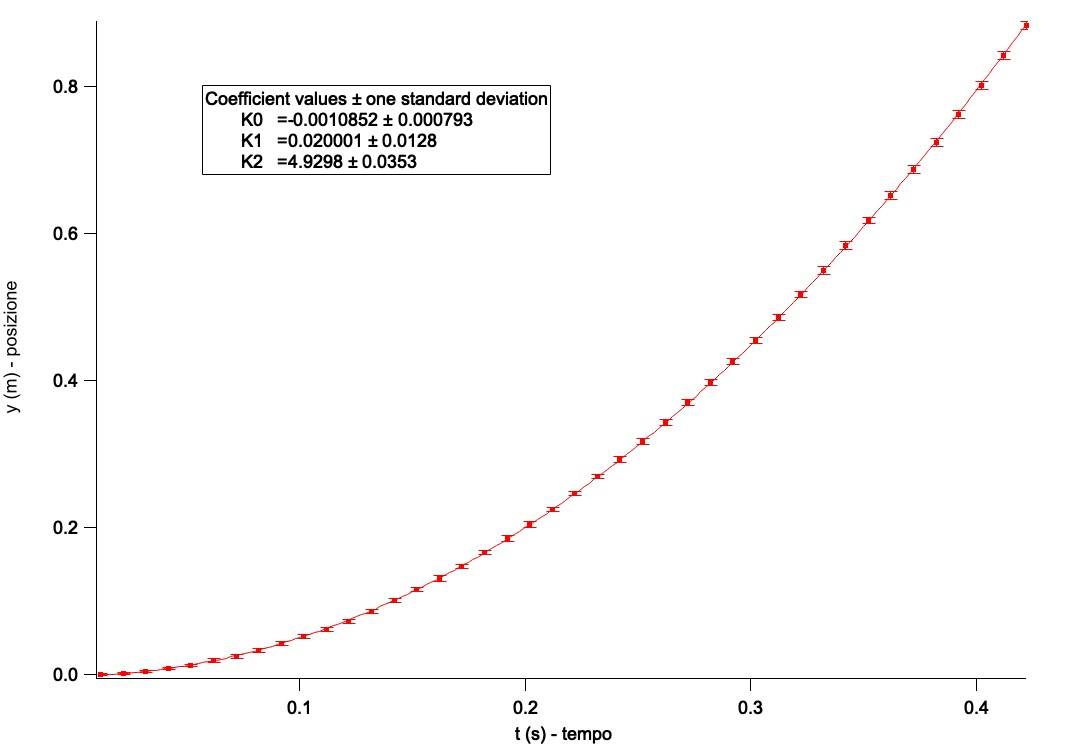
\includegraphics[width=170mm]{Immagini/Graph4 non comp.jpg}
\caption{\textit{{\footnotesize{Grafico $y_{mis}(t)$:  Sulle ordinate compaiono i valori delle poszioni misurate $y_{mis}$, associati ai relativi errori  \textit{$\Delta y^{'}$}, mentre sulle ascisse gli istanti di tempo \textit{t}}}}}
\label{Grafico parabolico}
\end{figure}

I dati ottenuti tramite la regressione di potenza del secondo ordine (\textit{poli 3}), non sono compatibili con i valori attesi, fatta eccezione per $\displaystyle{\frac{g}{2}}$.

    \bigskip
Visto che \textit{posizione iniziale} e \textit{velocità iniziale} non sono compatibili con i valori attesi si è corretta l'incompatibilità, isolando a destra il termine in relazione  quadratica con il tempo, mentre a sinistra, si è ottenuta una nuova variabile $y_{new}$ in cui, la posizione $y_{mis}$, è corretta dai termini $K_0$ e $ K_1\ t$, col rispettivo errore $\Delta y_{new}$: \\
L'equazione diventa quindi:
\begin{equation*}
\begin{aligned}
  & & (y_{mis} - K_0 - K_1\ t) = K_0'+K_1'\ t+K_{2}'\ t^2
  &\quad{} 
  \end{aligned}
  \begin{aligned}
  & &\text{dove:\phantom{.......}} y_{new} = y_{mis} - K_0 - K_1\ t 
  &
  \end{aligned}
\end{equation*}
L'errore su  $y_{new}$ è dato da
\begin{equation*}
 \Delta y_{new} = \Delta y^{'} + \Delta K_0 + \sqrt{\left(\frac{\Delta K_1}{K_1}\right)^2 + \left(\frac{\Delta t}{t}\right)^2}
 \end{equation*}
\\
\\
\\
\begin{longtable}{|c|c|}
    \hline
    \multirow{2}{*}{\small Misura} &
    \multirow{2}{*}{ \small$y_{new}\pm \Delta y_{new}$\ $(m)$} 
    \\&\\
\hline
\hline
    \footnotesize $1$ & \footnotesize$0.001\pm0.002$\\ 
    \footnotesize $2$ & \footnotesize$0.003\pm0.002 $\\ 
    \footnotesize $3$ & \footnotesize$0.005\pm0.003 $\\
    \footnotesize $4$ & \footnotesize$0.009\pm0.003 $\\
    \footnotesize $5$ & \footnotesize$0.013\pm0.003 $\\
    \footnotesize $6$ & \footnotesize$0.019\pm0.004$\\
    \footnotesize $7$ & \footnotesize$0.025\pm0.004$\\
    \footnotesize $8$ & \footnotesize$0.032\pm0.005$\\
    \footnotesize $9$ & \footnotesize$0.041\pm0.004$\\  
    \footnotesize $10$ & \footnotesize$0.051\pm0.005$\\
    \footnotesize $11$ & \footnotesize$0.061\pm0.004$\\
    \footnotesize $12$ &\footnotesize $0.072\pm0.006$\\
    \footnotesize $13$ & \footnotesize$0.085\pm0.006$\\
    \footnotesize $14$ & \footnotesize$0.099\pm0.006$\\
    \footnotesize $15$ & \footnotesize$0.114\pm0.006$\\
    \footnotesize $16$ & \footnotesize$0.129\pm0.006$\\
    \footnotesize $17$ & \footnotesize$0.145\pm0.006$\\
    \footnotesize $18$ & \footnotesize$0.163\pm0.006$\\
    \footnotesize $19$ & \footnotesize$0.182\pm0.007$\\
    \footnotesize $20$ & \footnotesize$0.201\pm0.007$\\
    \footnotesize $21$ & \footnotesize$0.222\pm0.006$\\
    \footnotesize $22$ & \footnotesize$0.243\pm0.007$\\ 
    \footnotesize $23$ & \footnotesize$0.266\pm0.007$\\
    \footnotesize $24$ & \footnotesize$0.290\pm0.008$\\
    \footnotesize $25$ & \footnotesize$0.314\pm0.008$\\
    \footnotesize $26$ & \footnotesize$0.339\pm0.008$\\
    \footnotesize $27$ & \footnotesize$0.366\pm0.008$\\
    \footnotesize $28$ & \footnotesize$0.393\pm0.009$\\
    \footnotesize $29$ & \footnotesize$0.421\pm0.008$\\
    \footnotesize $30$ & \footnotesize$0.450\pm0.009$\\
    \footnotesize $31$ & \footnotesize$0.481\pm0.009$\\
    \footnotesize $32$ & \footnotesize$0.513\pm0.009$\\
    \footnotesize $33$ & \footnotesize$0.544\pm0.010$\\  
    \footnotesize $34$ & \footnotesize$0.578\pm0.010$\\
    \footnotesize $35$ & \footnotesize$0.612\pm0.010$\\
    \footnotesize $36$ & \footnotesize$0.646\pm0.011$\\
    \footnotesize $37$ & \footnotesize$0.681\pm0.011$\\
    \footnotesize $38$ & \footnotesize$0.718\pm0.011$\\
    \hline
    \footnotesize $39$ & \footnotesize$0.756\pm0.011$\\
    \footnotesize $40$ & \footnotesize$0.795\pm0.012$\\
    \footnotesize $41$ & \footnotesize$0.835\pm0.011$\\
    \footnotesize $42$ & \footnotesize$0.876\pm0.011$\\
    \hline 
  \caption{\begin{footnotesize}
      Sono riportati in Tabella la posizione corretta $y_{new}$ ed il rispettivo errore $\Delta y_{new}$.
  \end{footnotesize}}
  \label{tab: ynew e errore}
\end{longtable}

Facendo una nuova regressione di potenza del secondo ordine utilizzando i nuovi dati, si ottene che le variabili $K_0'$, $K_1'$ e $K_2'$ sono tutte compatibili, come possiamo vedere in Figura \ref{Grafico parabolico}:
\bigskip
\bigskip

    \begin{figure}[h!]
\centering
\includegraphics[width=170mm]{Immagini/Grafico t-2.jpg}
\caption{\textit{{\footnotesize{Grafico $y_{new}(t)$:  Sulle ordinate compaiono i valori delle poszioni corrette $y_{new}$, associati ai relativi errori  \textit{$\Delta y_{new}$}, mentre sulle ascisse gli istanti di tempo \textit{t}}}}}
\label{Grafico parabolico}
\end{figure}
  
  



\section{Regressione lineare}
Successivamente si è fatta una regressione lineare, partendo da $y_{new}= \frac{1}{2}\ g t^2$, approssimando posizione e velocità iniziali a $0$. Quello che ci si aspetta di trovare è che la posizione sia in relazione quadratica con il tempo.

Posti

\phantom{aad} $ln{(A)}=a$ \phantom{aad} , \phantom{aad} $B=b$
\begin{equation*}
\begin{aligned}
  & y_{new}= A\ t^B
  &\quad{} 
  \end{aligned}
  \begin{aligned}
  &&\text{passando ai logaritmi:\phantom{..}}& & \ln{(y_{new})}=a +b\ \ln{(t)}
  &
  \end{aligned}
\end{equation*}

e come errore su $\ln({y_{new}})$: 
\begin{equation*}
    \Delta\ln{(y_{new})}=\frac{\Delta y_{new}}{y_{new}}\ 
\end{equation*}\\
\\
\\
\begin{longtable}{|c|c|c|}
    \hline
    \multirow{2}{*}{\small Misura} 
    &\multirow{2}{*}{\small$\ln({y_{new}}) \pm\Delta\ln{(y_{new})}$\ $(m)$} 
    &\multirow{2}{*}{\small$ln(t)\pm\Delta ln(t)$} 
    \\
    &&
    \\
    \hline
    \footnotesize$1$ & \footnotesize$-7.00\pm2.00$  &\footnotesize$-4.422\pm 0.080$\\
    \footnotesize$2$ & \footnotesize$-5.90\pm0.90$&\footnotesize$-3.821\pm 0.050$  \\
    \footnotesize$3$ & \footnotesize$-5.30\pm0.60$&\footnotesize$-3.442\pm 0.030$  \\
    \footnotesize$4$ & \footnotesize$-4.70\pm0.40$ &\footnotesize$-3.170\pm 0.020$ \\
    \footnotesize$5$ & \footnotesize$-4.30\pm0.30$&\footnotesize$-2.966\pm 0.020$  \\
    \footnotesize$6$ & \footnotesize$-3.90\pm0.20$&\footnotesize$-2.780\pm 0.020$  \\
    \footnotesize$7$ & \footnotesize$-3.80\pm0.20$ &\footnotesize$-2.631\pm 0.010$ \\
    \footnotesize$8$ & \footnotesize$-3.40\pm0.20$&\footnotesize$-2.501\pm 0.010$   \\
    \footnotesize$9$ & \footnotesize$-3.20\pm0.10$&\footnotesize$-2.390\pm 0.010$   \\
    \footnotesize$10$ & \footnotesize$-3.00\pm0.09$&\footnotesize$-2.282\pm 0.009$ \\
    \footnotesize$11$ & \footnotesize$-2.80\pm0.07$&\footnotesize$-2.190\pm 0.008$ \\
    \footnotesize$12$ & \footnotesize$-2.64\pm0.08$&\footnotesize$-2.103\pm 0.008$ \\
    \footnotesize$13$ & \footnotesize$-2.47\pm0.07$&\footnotesize$-2.024\pm 0.007$ \\
    \footnotesize$14$ & \footnotesize$-2.32\pm0.06$&\footnotesize$-1.951\pm 0.007$ \\
    \footnotesize$15$ & \footnotesize$-2.17\pm0.05$&\footnotesize$-1.883\pm 0.006$ \\
    \footnotesize$16$ & \footnotesize$-2.05\pm0.05$&\footnotesize$-1.820\pm 0.006$ \\
    \footnotesize$17$ & \footnotesize$-1.93\pm0.04$&\footnotesize$-1.760\pm 0.005$ \\
    \footnotesize$18$ & \footnotesize$-1.81\pm0.04$&\footnotesize$-1.703\pm 0.005$ \\
    \footnotesize$19$ & \footnotesize$-1.70\pm0.04$&\footnotesize$-1.650\pm 0.005$ \\
    \footnotesize$20$ & \footnotesize$-1.60\pm0.04$&\footnotesize$-1.609\pm 0.005$ \\
    \footnotesize$21$ & \footnotesize$-1.51\pm0.03$&\footnotesize$-1.551\pm 0.005$ \\
    \footnotesize$22$ & \footnotesize$-1.41\pm0.03$&\footnotesize$-1.515\pm 0.004$ \\
    \footnotesize$23$ & \footnotesize$-1.32\pm0.03$&\footnotesize$-1.461\pm 0.004$ \\
    \footnotesize$24$ & \footnotesize$-1.24\pm0.03$&\footnotesize$-1.429\pm 0.004$ \\
    \footnotesize$25$ & \footnotesize$-1.16\pm0.03$&\footnotesize$-1.388\pm 0.004$ \\
    \footnotesize$26$ & \footnotesize$-1.08\pm0.02$&\footnotesize$-1.349\pm 0.004$ \\
    \footnotesize$27$ & \footnotesize$-1.01\pm0.02$&\footnotesize$-1.302\pm 0.004$ \\
    \footnotesize$28$ & \footnotesize$-0.93\pm0.02$&\footnotesize$-1.276\pm 0.003$ \\
    \footnotesize$29$ & \footnotesize$-0.86\pm0.02$&\footnotesize$-1.231\pm 0.003$ \\
    \footnotesize$30$ & \footnotesize$-0.80\pm0.02$&\footnotesize$-1.207\pm 0.003$ \\
    \footnotesize$31$ & \footnotesize$-0.73\pm0.02$&\footnotesize$-1.165\pm 0.003$ \\
    \footnotesize$32$ & \footnotesize$-0.67\pm0.02$&\footnotesize$-1.133\pm 0.003$ \\
    \footnotesize$33$ & \footnotesize$-0.61\pm0.02$&\footnotesize$-1.103\pm 0.003$ \\
    \footnotesize$34$ & \footnotesize$-0.55\pm0.02$&\footnotesize$-1.073\pm 0.003$ \\
    \footnotesize$35$ & \footnotesize$-0.50\pm0.02$&\footnotesize$-1.044\pm 0.003$\\
    \footnotesize$36$ & \footnotesize$-0.44\pm0.02$&\footnotesize$-1.026\pm 0.003$ \\
    \footnotesize$37$ & \footnotesize$-0.38\pm0.02$&\footnotesize$-0.990\pm 0.003$ \\
    \footnotesize$38$ & \footnotesize$-0.33\pm0.02$&\footnotesize$-0.962\pm 0.003$ \\
    \hline
    \hline
    \footnotesize$39$ & \footnotesize$-0.28\pm0.02$&\footnotesize$-0.940\pm 0.002$ \\
    \footnotesize$40$ & \footnotesize$-0.23\pm0.02$&\footnotesize$-0.911\pm 0.002$ \\ 
    \footnotesize$41$ & \footnotesize$-0.18\pm0.01$&\footnotesize$-0.890\pm 0.002$ \\
    \footnotesize$42$ & \footnotesize$-0.13\pm0.01$&\footnotesize$-0.863\pm 0.002$ \\
    \hline
        \caption{\begin{footnotesize}
            Sono riportati in Tabella il logartimo della posizione $ln(y_{new})$ e il logaritmo del tempo $ln(t)$ con i rispettivi errori.
        \end{footnotesize}}
        \label{tab:logaritmi con errore}
\end{longtable}
\bigskip


 Tramite \textit{Igor Pro} si è ottenuto il seguente grafico:\\
   \begin{figure}[h!]
\centering
\includegraphics[width=170mm]{Immagini/GraficoLn.jpg}
\caption{\textit{{\footnotesize{Grafico $\ln{(y_{new})}(\ln{(t)})$: sul'asse asse $y$ sono riportati i valori di $\ln{(y_{new})}$ coi rispettivi errori, sull'asse $x$ il $\ln{(t)}$}}}}
\label{Grafico logaritmico}
\end{figure}



Il valore di $b$ è compatibile col valore $2$, esponente del tempo nella formula usata in partenza.  Si è così dimostrato che vi è una relazione quadratica tra $y_{new}$ e $t$.



\section{Calcolo dell'accelerazione di gravità}

A questo punto, dopo aver verificato che la posizione iniziale e finale sono approssimabili a zero e che la posizione è in relazione quadrtica con il tempo, si può creare un grafico lineare con i valori $y_{new}$, coi rispettivi errori, sull'asse delle ordinate, e del tempo al quadrato su quello delle ascisse, così da essere in grado di ricavare il valore dell'accelerazione di gravità a partire dalla pendenza della retta ottenuta. I dati utilizzati sono riportati nella seguente tabella:

\bigskip

\bigskip

\bigskip
\begin{table}[h!]

\centerline{\begin{tabular}{|c|c|c|}
   \hline
   
    \multirow{2}{*}{\small Misura} 
    &\multirow{2}{*}{\small $y_{new}\pm\Delta y_{new}$\ $(m)$}
    &\multirow{2}{*}{\small $t^2\pm \Delta t^2 (s)$}
    \\
    & &
    \\
    \hline
    \footnotesize $1$ & \footnotesize$0.001\pm0.002$ & \footnotesize$0.000\pm0.002$\\ 
    \footnotesize $2$ & \footnotesize$0.003\pm0.002 $ & \footnotesize$0.001\pm0.002$\\ 
    \footnotesize $3$ & \footnotesize$0.005\pm0.003 $ & \footnotesize$0.001\pm0.002$\\
    \footnotesize $4$ & \footnotesize$0.009\pm0.003 $ & \footnotesize$0.002\pm0.002$\\
    \footnotesize $5$ & \footnotesize$0.013\pm0.003 $ & \footnotesize$0.003\pm0.002$\\
    \footnotesize $6$ & \footnotesize$0.019\pm0.004 $ & \footnotesize$0.004\pm0.002$\\
    \footnotesize $7$ & \footnotesize$0.025\pm0.004 $ & \footnotesize$0.005\pm0.002$\\
    \footnotesize $8$ & \footnotesize$0.032\pm0.005 $ & \footnotesize$0.007\pm0.002$\\
    \footnotesize $9$ & \footnotesize$0.041\pm0.004 $ & \footnotesize$0.008\pm0.002$\\  
    \footnotesize $10$ & \footnotesize$0.051\pm0.005$ & \footnotesize$0.010\pm0.002$\\
    \footnotesize $11$ & \footnotesize$0.061\pm0.004$ & \footnotesize$0.013\pm0.002$\\
    \footnotesize $12$ &\footnotesize $0.072\pm0.006$ & \footnotesize$0.015\pm0.002$\\
    \footnotesize $13$ & \footnotesize$0.085\pm0.006$ & \footnotesize$0.017\pm0.002$\\
    \footnotesize $14$ & \footnotesize$0.099\pm0.006$ & \footnotesize$0.020\pm0.002$\\
    \footnotesize $15$ & \footnotesize$0.114\pm0.006$ & \footnotesize$0.023\pm0.002$\\
    \footnotesize $16$ & \footnotesize$0.129\pm0.006$ & \footnotesize$0.026\pm0.002$\\
    \footnotesize $17$ & \footnotesize$0.145\pm0.006$ & \footnotesize$0.030\pm0.002$\\
    \footnotesize $18$ & \footnotesize$0.163\pm0.006$ & \footnotesize$0.033\pm0.002$\\
    \footnotesize $19$ & \footnotesize$0.182\pm0.007$ & \footnotesize$0.037\pm0.002$\\
    \footnotesize $20$ & \footnotesize$0.201\pm0.007$ & \footnotesize$0.041\pm0.002$\\
    \footnotesize $21$ & \footnotesize$0.222\pm0.006$ & \footnotesize$0.046\pm0.002$\\
    \footnotesize $22$ & \footnotesize$0.243\pm0.007$ & \footnotesize$0.049\pm0.002$\\ 
    \footnotesize $23$ & \footnotesize$0.266\pm0.007$ & \footnotesize$0.054\pm0.002$\\
    \footnotesize $24$ & \footnotesize$0.290\pm0.008$ & \footnotesize$0.059\pm0.002$\\
    \footnotesize $25$ & \footnotesize$0.314\pm0.008$ & \footnotesize$0.064\pm0.002$\\
    \footnotesize $26$ & \footnotesize$0.339\pm0.008$ & \footnotesize$0.069\pm0.002$\\
    \footnotesize $27$ & \footnotesize$0.366\pm0.008$ & \footnotesize$0.074\pm0.002$\\
    \footnotesize $28$ & \footnotesize$0.393\pm0.009$ & \footnotesize$0.080\pm0.002$\\
    \footnotesize $29$ & \footnotesize$0.421\pm0.008$ & \footnotesize$0.085\pm0.002$\\
    \footnotesize $30$ & \footnotesize$0.450\pm0.009$ & \footnotesize$0.091\pm0.002$\\
    \footnotesize $31$ & \footnotesize$0.481\pm0.009$ & \footnotesize$0.097\pm0.002$\\
    \footnotesize $32$ & \footnotesize$0.513\pm0.009$ & \footnotesize$0.104\pm0.002$\\
    \footnotesize $33$ & \footnotesize$0.544\pm0.010$ & \footnotesize$0.110\pm0.002$\\  
    \footnotesize $34$ & \footnotesize$0.578\pm0.010$ & \footnotesize$0.117\pm0.002$\\
    \footnotesize $35$ & \footnotesize$0.612\pm0.010$ & \footnotesize$0.124\pm0.002$\\
    \footnotesize $36$ & \footnotesize$0.646\pm0.011$ & \footnotesize$0.131\pm0.002$\\
    \footnotesize $37$ & \footnotesize$0.681\pm0.011$ & \footnotesize$0.138\pm0.002$\\
    \footnotesize $38$ & \footnotesize$0.718\pm0.011$ & \footnotesize$0.146\pm0.002$\\
    \footnotesize $39$ & \footnotesize$0.756\pm0.011$ & \footnotesize$0.154\pm0.002$\\
    \footnotesize $40$ & \footnotesize$0.795\pm0.012$ & \footnotesize$0.162\pm0.002$\\
    \footnotesize $41$ & \footnotesize$0.835\pm0.011$ & \footnotesize$0.170\pm0.002$\\
    \footnotesize $42$ & \footnotesize$0.876\pm0.011$ & \footnotesize$0.178\pm0.002$\\
    \hline
    \end{tabular}}
        \caption{\begin{footnotesize}
            Sono riportati in Tabella la posizione $y_{new}$ ed il tempo al quadrato $t^2$ con i rispettivi errori.
        \end{footnotesize}}
        \label{tab:posizione corr tempo quadro non comp}
\end{table}


\newpage

Il grafico ottenuto è il seguente:

  \begin{figure}[h!]
\centering
\includegraphics[width=170mm, height=80mm]{Immagini/Grafico t^2-1.jpg}
\caption{\textit{{\footnotesize{Grafico $y_{new}(t^2)$: sull'asse asse $y$ sono riportati i valori di $y_{new}$ coi rispettivi errori, sull'asse $x$ il tempo al quadrato}}}}
\label{Grafico logaritmico}
\end{figure}



Dove $\displaystyle b=\frac{1}{2}\ g=(4.9301\pm 0.0216)$, da cui:
\begin{equation*}
    g=2 \ b=9.8602 \ \frac{m}{s^2}
\end{equation*}
e l'errore è
\begin{equation*}
    \Delta g=2\ \Delta b=0.0432\approx 0.04 \ \frac{m}{s^2}
\end{equation*}

\addvspace{1.5cm}
Quindi l'accelerazione di gravità ottenuta sarebbe $g=(9.86\pm0.04)$ $\frac{m}{s^2}$.
Il valore $g$, ottenuto a partire da $b$ , non risulta compatibile col valore standard, poichè $|g-g_{tab}|> |\Delta g-\Delta g_{tab}|$. Questo è dovuto al fatto che ci potrebbero essere errori dovuti alla configurazione e alla qualità video dell'esperimento, che non erano sotto il nostro controllo.

\addvspace{10cm}
Per queste ragioni si è passati a due deviazioni standard con una confidenza del 95\%, e il grafico ottenuto è il seguente:

\addvspace{1.5cm}
  \begin{figure}[h!]
\centering
\includegraphics[width=170mm, height=80mm]{Immagini/Graficot^2-2.jpg}
\caption{\textit{{\footnotesize{Grafico $y_{new}(t^2)$: sull'asse asse $y$ sono riportati i valori di $y_{new}$ coi rispettivi errori, sull'asse $x$ il tempo al quadrato}}}}
\label{Grafico compatibile y(t^2)}
\end{figure}





Si è infine passati al calcolo di $g$, utilizzando come errore su $b$ il nuovo valore $\Delta b=0.0436$:
\begin{equation*}
    g=2 \ b=9.8602\ \frac{m}{s^2}
\end{equation*}
e l'errore è
\begin{equation*}
    \Delta g=2\ \Delta b=0.0872\approx 0.09\ \frac{m}{s^2}
\end{equation*}
Quindi il valore dell'accelerazione di gravità risultate è $g=(9.86\pm0.09)$ $\frac{m}{s^2}$
\section{Compatibilità}
Confrontiamo questo risultato col dato dell'accelerazione di gravità tabulato $g_{tab}=(9.80665\pm 0.00001)\ m/s^2$, trascurandone l'errore poichè molto inferiore rispetto a quello calcolato:
\begin{equation*}
\begin{aligned}
  & |g-g_{tab}|=0.05335 \ \frac{m}{s^2}
  &\quad{} 
  \end{aligned}
  \begin{aligned}
  &&\text{,\phantom{..}}& & 
  |\Delta g-\Delta g_{tab}|=0.09\ \frac{m}{s^2}
  &
  \end{aligned}
\end{equation*}

Visto che $|g-g_{tab}|<< |\Delta g-\Delta g_{tab}|$, il valore trovato è compatibile col valore standard.

\newpage
\section{Conclusioni}
La prima difficoltà è stata riscontrata nello stabilire tramite il programa di tracciamento le \\
distanze metriche del video perchè, nonostante l'asta presentasse ogni 10cm un segno, questi erano tutt'altro che sottili, e ciò ha contribuito alle non compatibilità riscontrate successivamente. 

Anche in prossimità della fine della caduta è stato difficile prendere dei dati accurati, perchè non era chiaro quando la sfera colpisse il tavolo, quindi, per evitare di misurare ad urto avvenuto, si è effettuata l'ultima misura quando si era sicuri che fosse ancora in moto.

Infatti, nella prima regressione lineare, nè la velocità iniziale nè l'ordinata iniziale sono compatibili con i valori attesi di 0. Sono stati resi compatibili correggendole, come mostrato nel paragrafo \ref{Agg. misure xconcl}: \textit{Regressione di potenza}.\\

Per quanto riguarda la misura di $g$, inizialmente si era calcolato un errore relativo $\frac{\Delta g}{g}\approx 6\% $ ottenuto a partire da dei valori intermedi delle nostre misure. L'errore relativo dell'accelerazione di gravità calcolata alla fine è:

\begin{equation*}
    \frac{\Delta g}{g}=\frac{0.09}{9.86}=0.9\%
\end{equation*}
risultato che differisce di un ordine di grandezza dal primo. Questo può essere dovuto al fatto che si è cosiderato un errore specifico per ogni misura, in base alla definizione del frame, quindi alcune misure risultano più precise di altre. Inoltre sono state attuate le correzioni citate prima, per rendere compatibili  la posizione iniziale e la velocità iniziale. \\


Successivamente si è effettuata una regressione di potenza sulla relazione che intercorre tra la posizione e tempo. L'esponente risulta pienamente compatibile con il valore atteso di 2, calcolato con una deviazione standard.
Per il calcolo di $g$, invece, si è usata una regressione lineare tra posizione e tempo al quadrato, per la quale è stato necessario aumentare la confidenza al 95\% (2 deviazioni standard) perchè il valore di $g$ ottenuto inizialmente non era compatibile. \\

Nonostante tutti i risultati, alla fine, siano corretti, si sarebbero potute migliorare le stime agendo sulla calibrazione dello strumento di misura su Tracker, che  probabilmente è la fonte di errore maggiore. Considerando la distanza tra più di 2 segni sulla sbarra (ad esempio calibrando su $30cm$ invece di $10cm$), l'errore effettivo (non quello stimato) sarebbe calato e quindi si sarebbero avute misure più attendibili.
Inoltre, date le incompatibilità riscontrate, e anche l'errore molto piccolo risultante su $g$, può essere che gli errori sulle singole misure fossero stati sottostimati.






\end{document}
